\chapter{Stato dell'arte}\label{ch:theory}
%In questo capitolo sono introdotti a livello teorico i concetti necessari per la comprensione del lavoro svolto
\section{Immagini fake: rischi, generazione e rilevamento}\label{sec:fakeimg}
L'incremento degli studi nel campo dei modelli generativi, ossia tecniche di intelligenza artificiale dedicate alla generazione di dati simili a quelli di addestramento, ha portato allo sviluppo di tecnologie in grado di produrre immagini indistinguibili da quelle reali; la diffusione al pubblico di questi strumenti rende la creazione di immagini sintetiche con alto livello di realismo un'operazione semplice ed accessibile anche a utenti non esperti.\\ 
Tra le immagini false si possono distinguere due categorie principali: \textit{cheapfakes}, tecniche di manipolazione meno sofisticate, come \textit{splicing} e \textit{copy-move}, e  \textit{deepfakes}, metodi che fanno uso di intelligenza artificiale.\\Il termine deepfake nasce dalla combinazione di "deeplearning" e "fake" e vuole indicare la manipolazione di contenuti già esistenti o la generazione di nuovi tramite l'utilizzo di modelli di deeplearning. L'attenzione di questo lavoro sarà concentrata su quest'ultima categoria.\\
L'uso più comune dei deepfakes riguarda la produzione e rielaborazione di immagini rappresentanti volti umani, con applicazioni nel mondo dell'intrattenimento o del marketing; le stesse tecnologie possono però essere utilizzate per fini illeciti come la creazione di profili falsi ma apparentemente autentici, diffusione di disinformazione e produzione di materiale diffamatorio nei confronti di personaggi pubblici o privati.
%\textit{esempi??}
\paragraph{Manipolazioni di volti} Tra le più comuni manipolazioni si trovano \cite{tolosana2020deepfakes}:
\textit{entire face synthesis}, ossia la creazione di immagini di volti di persone non reali; \textit{identity swap}, che consiste nella sostituzione del volto di un individuo con quello di un altro; \textit{attribute manipulation}, ovvero la modifica di attributi/caratteristiche del volto e \textit{expression swap}, che ha lo scopo di modificare l'espressione facciale della persona scelta. Nella figura \ref{fig:facemanip} sono mostrati esempi per ogni tipo di manipolazione.
Questo lavoro si concentra sulla \textit{entire face synthesis} e ci riferiremo principalmente a questa parlando di generazione e identificazione  di immagini sintetiche.
\begin{figure}
    \centering
     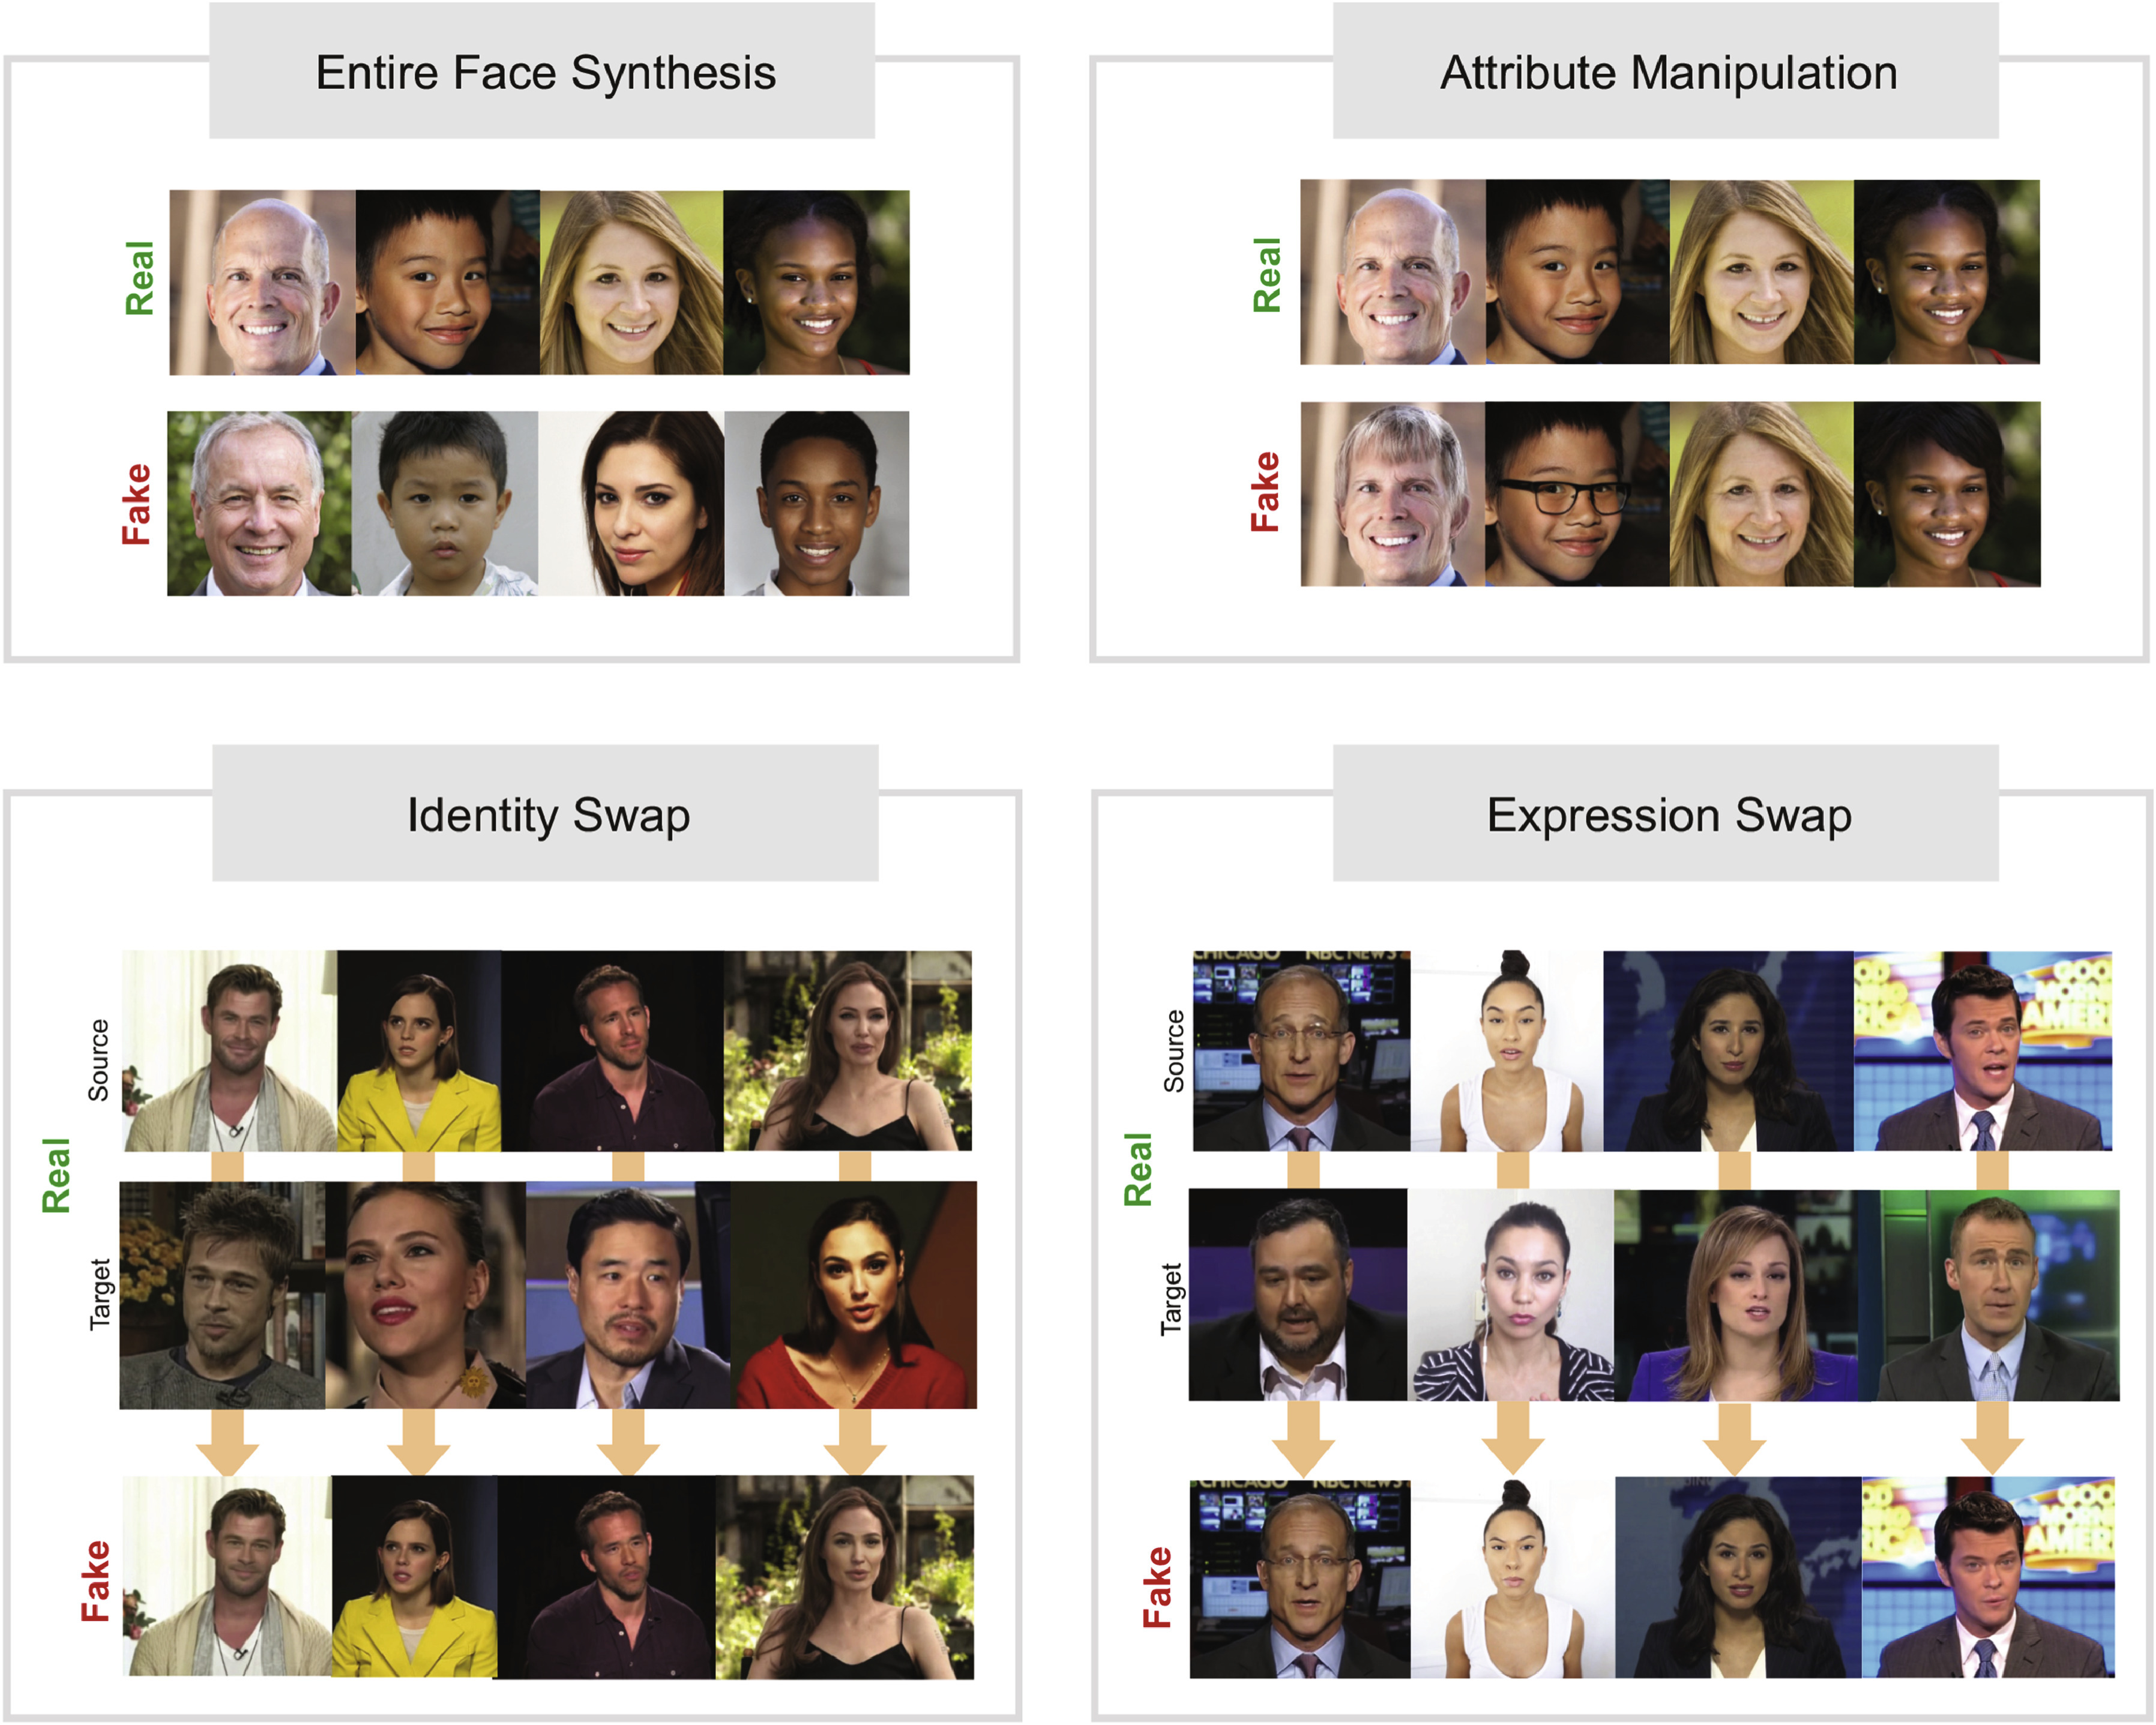
\includegraphics[width=1\linewidth]{img/face manipulations.jpg}
     \caption{Esempi per ogni tipo di manipolazione su immagini di volti}
     \label{fig:facemanip}
\end{figure}
\subsection{Generazione}
I modelli generativi  hanno l'obbiettivo di apprendere la distribuzione dei dati di addestramento e trovare il miglior modo per rappresentarli in modo da generare nuovi campioni simili a quelli originali.
Per la creazione di immagini di volti sintetiche sono usate principalmente tre architetture \cite{fernando2025face}: Autoencoders, Diffusion Models e GANs. Comprenderne il funzionamento è fondamentale per sviluppare metodi di identificazione.
\paragraph{Autoencoders} Sono architetture composte da un encoder, che ha l'obbiettivo di trasformare l'input in una rappresentazione latente compatta, ed un decoder che ricostruisce l'immagine desiderata. Sono spesso usate nell'identity swapping sfruttando un encoder comune che apprende una rappresentazione latente condivisa, e decoder separati che si specializzano nella ricostruzione di immagini relative ad un individuo specifico \cite{fernando2025face}, così da ottenere uno scambio di identità decodificando la rappresentazione compatta della persona $A$ con il decoder della persona $B$.
\paragraph{Diffusion Models} I modelli di diffusione sono modelli generativi il cui funzionamento si basa su due fasi: nel \textit{forward process} un'immagine reale viene corrotta introducendo rumore in un determinato numero di iterazioni; successivamente nel \textit{reverse process} il modello viene addestrato a sintetizzare un'immagine realistica rimuovendo progressivamente rumore da rumore puro \cite{ho2020denoising}. L'approccio iterativo di queste fasi permette di generare immagini di alta qualità riuscendo a catturare dettagli fini; per questo i Diffusion Models  rappresentano attualmente lo stato dell'arte nel campo della generazione di immagini.
\subsection{GANs}\label{subsec:GAN}
GAN (\textit{Generative Adversarial Networks}) è l'architettura proposta nel 2014 da Goodfellow et al. \cite{goodfellow2014generative} composta da due reti neurali: generatore e discriminatore. Il generatore $G$ riceve in input rumore casuale $z$ e lo mappa in un'immagine sintetica $G(z)$; il discriminatore $D$ riceve in input immagini reali o sintetiche ed ha il compito di classificarle.
Le due reti vengono addestrate contemporaneamente competendo in un \textit{min-max game} nel quale $G$, generando immagini sempre più realistiche, ha l'obbiettivo di massimizzare la probabilità che $D$ compia un errore nella classificazione, mentre $D$ deve minimizzarla. L'equazione che descrive questo gioco è la seguente:
\begin{equation}
\min_G \max_D V(D,G) = \mathbb{E}_{x \sim p_{data}(x)} [\log D(x)] + \mathbb{E}_{z \sim p_z(z)} [\log(1 - D(G(z)))]
\end{equation}\label{eq:gan}
Durante l'addestramento il gradiente della funzione di perdita di $D$ verrà usato per aggiornare $G$. Inizialmente $G$ genererà immagini rumorose e facilmente identificabili come falsi da $D$, ma con il procedere della fase di addestramento la qualità delle immagini aumenterà fino a farle diventare abbastanza realistiche da ingannare $D$.\\
Questa architettura ha rappresentato il primo salto di qualità nel campo della generazione di immagini e per anni è stata  il punto di riferimento.
Di seguito viene approfondita la variante di GAN usata per creare il dataset di immagini sintetiche per gli esperimenti svolti (vedi sez \ref{sec:dataset}).
\paragraph{StyleGAN}\label{par:style}
StyleGAN \cite{karras2019style} presenta un'importante innovazione rispetto alla struttura classica: il generatore non riceve come input direttamente il rumore casuale $z$, ma questo viene prima trasformato da un mapping network $f : \mathcal{Z} \rightarrow \mathcal{W}$ in un vettore $f(z) = w$ in uno spazio latente intermedio $\mathcal{W}$ non vincolato dalla distribuzione del dataset di addestramento, proprietà che invece vincola $\mathcal{Z}$. Successivamente $w$ viene trasformato in una serie di stili $y$ che sono interpretati da ogni layer del generatore come istruzioni su come operare attraverso un'operazione chiamata \textit{Adaptive Instance Normalization} (AdaIN), controllando così il contributo di ogni layer alla generazione dell'immagine.\\L'architettura è visbile in fig. \ref{fig:stylegan}.
\begin{figure}
    \centering
    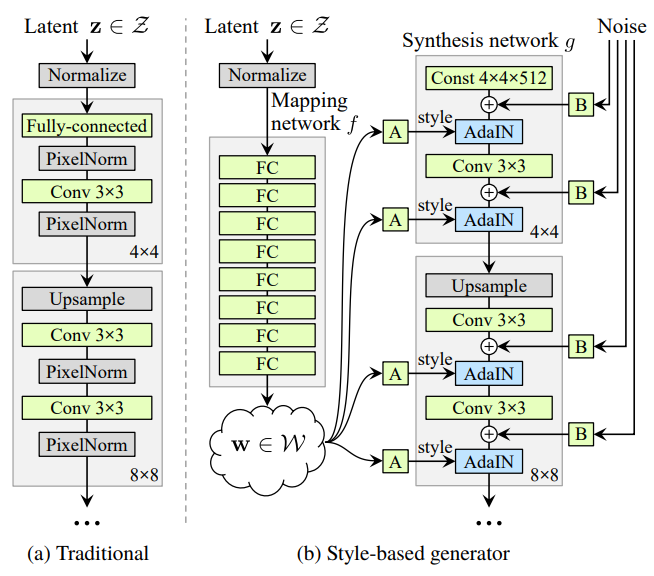
\includegraphics[width=1\linewidth]{img/style-arch.png} \caption{Architettura di StyleGAN descritta in \cite{karras2019style}}\label{fig:stylegan}
\end{figure}
L'innovazione di StyleGAN consiste quindi nel modo innovativo di generare immagini basandosi su una collezione di stili; in particolare gli effetti di ogni stile sono localizzati nella rete, permettendo di scegliere sottoinsiemi di stili per modificare solo alcuni aspetti dell'immagine.
Da notare come StyleGAN non modifica la struttura del discriminatore, che rimane quello classico, ma cambia il controllo e la qualità del generatore, permettendo di ottenere immagini più realistiche e con un maggior controllo sugli attributi generati.
% TODO leggere: https://onlinelibrary.wiley.com/doi/full/10.1111/cgf.14503?casa_token=qfRjy32wWI8AAAAA%3AL8TRQAh8tDCAhA-ve4k-Vu2Vv2sWzt4ZRxmfl2_kAsOZuEM6111KhlckpCk4HFsaOS6H8EEL14OPdA
\subsection{Rilevamento}
Data un'immagine $I$ un detector di immagine sintetiche ha il compito di rendere un valore chiamato detection score che indica la probabilità che $I$ sia sintetica.
La ricerca riguardante tecniche di rilevamento è in continuo sviluppo data la necessità di riuscire a contrastare le tecnologie di generazione sempre più sofisticate.
%Ogni immagine digitale può essere pensata come un insieme di caratteristiche che rappresentano la sua \textit{digital history}: processo di acquisizione, preprocessing interno alla camera, operazioni di editing o di post processing; queste possono essere sfruttate per trovare anomalie che possono indicare presenza di manipolazioni.
I metodi di rilevamento si possono suddividere in due categorie: quelli classici e quelli che sfruttano modelli di intelligenza artificiale.
\paragraph{Approcci classici}
I metodi di rilevamento classici si basano sull'analisi delle immagini in ricerca di anomalie create durante la fase di generazione.
I \textit{Physical-based methods} cercano di sfruttare inconsistenze nell'immagine, come illuminazione o il riflesso della luce negli occhi, che non sarebbero presenti in un'immagine reale. I \textit{Physiological-based Methods} invece investigano l'aspetto semantico, analizzando anomalie riguardanti l'asimmetria di attributi dei volti come diversi colori negli occhi, differenti forme delle pupille o un numero errato di denti.
Altri metodi invece cercano di trovare artefatti nelle caratteristiche "strutturali" delle immagini tra cui: imperfezioni causate dal sistema ottico delle fotocamere nel processo di acquisizione, processing interno o esterno alla fotocamera.\\
 Una caratteristica studiata è la PRNU (\textit{Photo Response Non-Uniformity}): ogni fotocamera lascia un pattern di rumore specifico nelle fotografie che può essere usato come una sorta di "impronta digitale"; l'assenza di questo pattern in una regione dell'immagine è un forte indicatore di manipolazione.\\
Allo stesso modo modelli generativi come GAN risultano lasciare degli artefatti chiamati "\textit{GAN fingerprint}" particolarmente riconoscibili analizzando le immagini nel dominio della frequenza per questo molti metodi classici analizzano lo spettro di Fourier.
\paragraph{Approcci basati su deeplearning} Gli approcci più recenti sfruttano il deep learning, usando reti neurali per estrarre le feature sulle quali fare le decisioni di classificazione in modo automatico.
Nel 2020 si è svolta la \textit{Kaggle Deepfake Detection Challenge} \cite{dolhansky2020deepfakedetectionchallengedfdc} , e le migliori soluzioni proposte erano basate su EfficientNet B7 \cite{pmlr-v97-tan19a} e XceptionNet \cite{8099678}.
Un'altra architettura molto usata è ResNet \cite{7780459}, che introduce il concetto di \textit{residual connetions} permettendo prestazioni superiori.
Recentemente i Vision transformer basati sulla self-attention, inizialmente  sviluppata per Natural Language Processing, sono stati usati in questo campo per la capacità di catturare relazioni globali nell'immagine.\\
Con l'avvento dei Diffusion Models alcuni ricercatori hanno provato a sviluppare tecniche basate sull'inversione del processo di diffusione sfruttando l'idea che l'immagine generata può essere riportata alla sua rappresentazione latente originale: facendo questo e ricostruendo l'immagine si possono analizzare gli errori di ricostruzione per la classificazione, e identificare immagini reali assumendo che dovrebbero presentare maggiori errori di ricostruzione \cite{wang2023dire}. 
\paragraph{Confronto tra i due approcci}
Gli approcci classici riescono ad ottenere buoni risultati su immagini non compresse, ma questa efficienza diminuisce drasticamente quando si lavora con immagini compresse, come quelle condivise sui social media, dove invece i metodi basati su deeplearning riescono a mantenere un buon livello di accuratezza. 
I metodi più recenti hanno però due svantaggi principali: il problema della non explainability, e della generalizzabilità.
La explainability è un requisito fondamentale nel campo della forensics, dato che la decisione di classificare un'immagine come sintetica deve essere motivata da prove concrete nel caso di ambiti legali.
Mentre come dimostrato in \cite{khodabakhsh2018fake}, nel rilevamento di \textit{Fake face images}, strumenti che risultano avere buone performance non riescono a generalizzare bene quando vengono testate su immagini sintetiche generate da tipi di architetture non presenti nel dataset di addestramento.
\newpage
\section{JPEG AI} \label{sec:jpegai}
La qualità e la risoluzione delle immagini  è in continua crescita, e così la loro dimensione in formato non compresso; considerando anche l'aumento del numero di immagini prodotte e visualizzate quotidianamente, si è sviluppata la necessità di trovare dei nuovi metodi di compressione in modo da consentire una trasmissione e un'archiviazione più efficienti.
Un nuovo promettente paradigma di compressione è chiamato"\textit{Learning-based image compression}" o "\textit{Neural image compression}" e sfrutta l'apprendimento automatico  facendo leva sulle reti neurali per raggiungere livelli di compressione maggiori.
\subsection{Compressione di immagini}
\begin{quote} 
    "\textit{A picture is worth a thousand words}"
\end{quote}
La compressione dei dati è un problema ampiamente studiato nell'informatica: l'obiettivo è quello di rappresentare un'informazione usando un numero ridotto di bit rispetto alla rappresentazione originale. Nel caso delle immagini questo equivale a rappresentare la stessa informazione visiva, almeno apparentemente, riducendo lo spazio di archiviazione utilizzato. La compressione si divide in due approcci: lossless,  senza perdita di informazione, e lossy, ovvero con perdita di informazione.\\
La compressione senza perdita viene utilizzata nelle applicazioni in cui è richiesta una perfetta ricostruzione dell'immagine originale, per esempio nel caso di immagini mediche. Quella con perdita viene usata per esempio nella condivisione delle immagini sul web perché consente di raggiungere un maggior livello di compressione scartando parte dell'informazione ma mantenendo una qualità accettabile.
\paragraph{Compressione lossy classica}
Tradizionalmente il processo per la compressione lossy prevede i seguenti passaggi: inizialmente viene applicata una trasformata all'immagine che mappa i pixel dal dominio spaziale ad uno più efficiente per la compressione, convertendoli in coefficienti. Questi vengono successivamente quantizzati, operazione nella quale avviene la principale perdita di informazione. Infine si effettua una codifica dell'entropia lossless per trasformare la sequenza di coefficienti quantizzati in un bitstream finale.\\
Il più importante e diffuso esempio di compressione lossy è JPEG \cite{jpeg}; il suo successo è dovuto al basso costo computazionale necessario per il calcolo della DCT (\textit{Trasformata discreta del coseno}), che, applicata a blocchi di $8 \times 8 $ pixel, mappa i pixel dal dominio spaziale a quello della frequenza, permettendo di concentrare la maggior parte dell'informazione rilevante in pochi coefficienti. Dopo questa trasformata i coefficienti vengono quantizzati in base alla loro frequenza, usando maggiore precisione per le frequenze più basse, che contengono più informazione per l'occhio umano, e approssimando maggiormente quelle più alte. \\
In generale le tecniche tradizionali sono state progettate "a mano" dai ricercatori sfruttando la conoscenza della struttura probabilistica dell'informazione, ed infatti fanno uso di una trasformata predeterminata e fissa, avendo lo svantaggio di non essere abbastanza flessibile e ottimale per tutti i tipi di immagine.
\subsection*{Learned image compression}
In questo nuovo paradigma vengono utilizzate le reti neurali: i primi articoli che propongono tecniche di questo tipo risalgono già agli anni '90 \cite{sonehara1989image, sicuranza1990artificial}, quando ancora la loro implementazione non era possibile nella pratica. Recentemente, con i progressi nell'apprendimento automatico e lo sviluppo di hardware specializzato come le GPU, anche il campo del learned image compression si è evoluto.\\
La differenza principale con i codec tradizionali come JPEG risiede nel fatto che in questo nuovo approccio ogni componente classica (trasformata, quantizzazione, codifica dell'entropia) è sostituita da una rete neurale, portando alla creazione di un \textit{learned image codec}.
%, ovvero reti neurali che apprendono trasformate \textit{non-lineari} permettendo una rappresentazione più adatta.
\paragraph{Architettura}La maggior parte delle tecniche sono basate sugli autoencoder \cite{theis2017lossy}, un tipo di rete neurale in grado di apprendere la mappatura tra l'input e uno spazio di una rappresentazione latente compatta, spesso chiamato \textit{bottleneck}.\\
L'architettura che ha riscosso più successo è quella proposta da \cite{balle2018variational} che ha dato prova dell'efficienza di questa tecnica, migliorata successivamente da \cite{minnen2018joint}.\\
Uno degli aspetti fondamentali è l'approccio end-to-end nel quale tutti i moduli, dall'encoder al decoder, vengono addestrati insieme mediante un'unica \textit{global loss-function} permettendo un'ottimizzazione "unificata" che massimizza l'efficienza di compressione. Questo rappresenta un vantaggio rispetto ai metodi tradizionali in cui ogni componente viene ottimizzata in modo indipendente.\\
Oltre agli autoencoder, si possono trovare anche altri tipi di architettura, e come proposto in \cite{ascenso2019report} si possono classificare in base a questi criteri:
\begin{itemize}
    \item tipologia di rete neurale utilizzata: oltre a quelli già citati, sono usate anche RNN, per elaborare l'immagine in modo sequenziale, oppure GAN (descritti in sez. \ref{subsec:GAN})
    \item dimensione dell'unità di codifica: alcune tecniche scelgono di elaborare l'intera immagine, mentre altre decidono di lavorare a blocchi di pixel riducendo la complessità
    \item strategia del controllo del bit rate: alcuni metodi scelgono di usare lo stesso modello per comprimere a più bitrate, altri invece utilzzano diversi modelli ottimizzati per un singolo livello di qualità
\end{itemize}
%TODO: per andare più nel dettaglio consultare anche sito Neuarl image compression in nutshell cap1
%TODO: nel sito si trova anche una spiegazione migliore di come si svolge l'allenamento
\subsection{Motivazioni per lo sviluppo di JPEG AI}
%TODO: leggere  "Learning based image coding", di JPEG che ha motivato sviluppo di JPEG AI
La principale motivazione dietro lo sviluppo è descritta nel seguente modo:
\begin{quote}
    "\textit{The scope of JPEG AI is to create a learning-based image coding standard that provides a single-stream, compact compressed domain representation targeting both human visualization,.., and effective performance for image processing and computer vision tasks, with the goal of supporting royalty-free baseline} \cite{ascenso2023jpegAI}"
\end{quote} L'obbiettivo può essere paragonato alla creazione di un "\textit{linguaggio comune}" che consenta una rappresentazione efficiente sia per la visione umana che per macchine. Questa scelta risulta rilevante considerando che ormai i contenuti digitali non sono più visualizzati solo dagli umani, ma in molte applicazioni, come sistemi di sorveglianza intelligente, sono le macchine i destinatari principali.
L'idea è quindi di usare la stessa rappresentazione compatta e ricca di informazione sia per task di \textit{image processing}, che \textit{computer vision}, oppure potrebbe essere ricostruita (vedi fig. \ref{fig:fig:jpeg_frw}) per renderla visibile ad un utente umano.\\
\begin{figure}
    \centering
    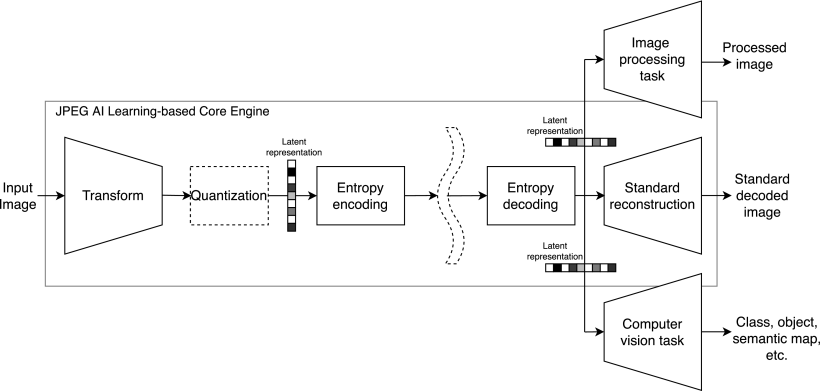
\includegraphics[width=1\linewidth]{img/JPEG AI.png}
    \caption{Framework JPEG AI}
    \label{fig:fig:jpeg_frw}
\end{figure}
Un unico bitstream multitask offre due vantaggi: il primo riguarda la riduzione della complessità necessaria a svolgere task di image processing o computer vision, consentendo di evitare completamente la parte di ricostruzione dell'immagine e di agire direttamente sulla rappresentazione latente. Il secondo vantaggio riguarda il potenziale incremento nell'accuratezza delle operazioni: essendo JPEG AI stato progettato, addestrato ed ottimizzato per trovare una rappresentazione compatta latente che riesca a contenere l'informazione (anche semantica) contenuta nell'immagine originale, svolgere task direttamente su questa potrebbe garantire prestazioni migliori rispetto ad utilizzare l'immagine lossy ricostruita, specialmente a bitrate bassi.\\
Per ottenere questo l'encoder di JPEG AI deve generare un bitstream indipendente da tutti task, ossia non ottimizzato per nessun compito specifico, mantenendo però il requisito fondamentale di un alto livello di compressione.
\subsection{Architettura}\label{sec:architetturaJPEGAI}
L'architettura di JPEG AI segue lo schema dei learning-based codec \cite{minnen2018joint} osservabile nella fig.\ref{fig:architmin}; si possono distinguere due moduli.
\begin{figure}
    \centering
    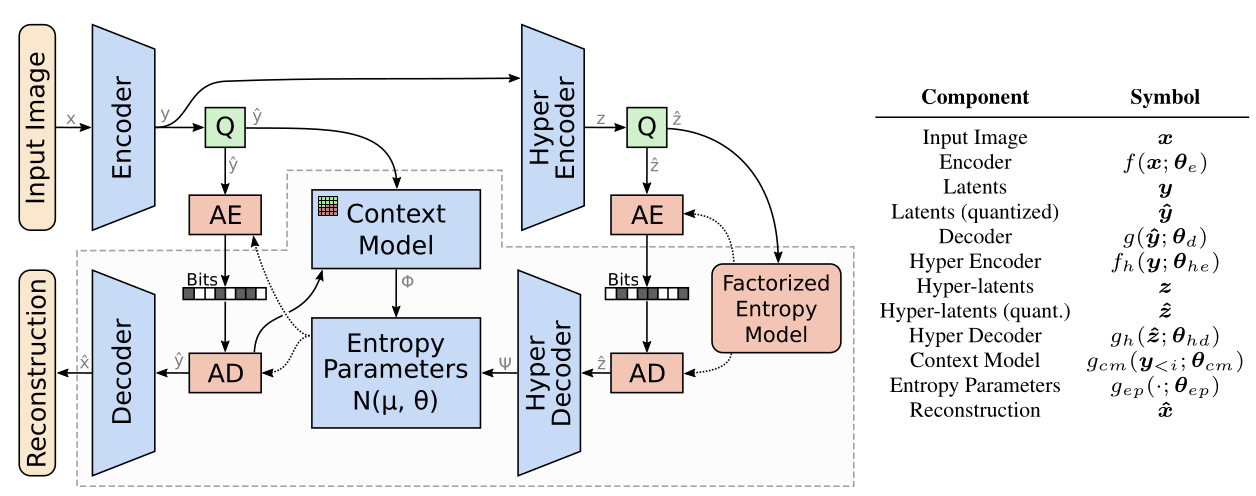
\includegraphics[width=1\linewidth]{img/architetturaJPEGAI.png}
    \caption{Architettura descritta in \cite{minnen2018joint}}
    \label{fig:architmin}
\end{figure}
Il modulo principale è rappresentato dall'autoencoder, composto dalla coppia \textit{encoder-decoder}. L'encoder apprende una trasformata non-lineare chiamata \textit{Analysis transform}, che mappa un'immagine $x$ in una rappresentazione latente più compatta $y$. Il decoder apprendende una trasformata non-lineare chiamata \textit{Synthesis transform} che ricostruisce un'approssimazione dell'immagine orginale partendo dalla versione quantizzata $\hat{y}$ della rappresentazione latente.\\
Il secondo modulo corrisponde al \textit{Modello per l'entropia}: composto da \textit{Hyperprior} e \textit{Context-model} apprende la distribuzione di probabilità dei valori dei tensori latenti per svolgere in modo più efficiente la codifica dell'entropia \cite{balle2018variational}. L'\textit{Hyperprior} è un autoencoder ausiliario composto da un \textit{hyper-encoder}, che estrae da $y$ delle \textit{side-information/hyper-latent} $z$ che vengono quantizzate ${(\hat{z})}$ ed incluse nel bitstream, ed un \textit{hyper-decoder}, che partendo $\hat{z}$ aiuta a predire la distribuzione dei valori del tensore latente. Il \textit{Context model}, utilizzando un approccio autoregressivo, usa il contesto dato dai valori già codificati $\hat{y}_{<i}$ per stimare la distribuzione dei valori.\\
\paragraph{Fase di Encoding}
Il processo di encoding di un'immagine si può osservare in \ref{fig:encodingJPEGAI}: inizialmente l'analysis transform, una rete neurale composta da layer convoluzionali e  attivazioni non lineari, trasforma l'immagine in un tensore latente $y$; questo viene elaborato dall'hyper-encoder che estrae da $y$ il tensore $z$, successivamente arrotondato ($\hat{z}$) e compresso nell'ultima parte del bitstream.
%Forse sarebbe meglio specificare cosa è ANS
Per la codifica entropica di $y$  viene usato un hyper-scale decoder, che riceve $\hat{z}$, e genera i parametri, per esempio le varianze, necessarie per descrivere la distribuzione di probabilità dei valori di $y$. Questi verranno usati per fare la codifica entropica dei residui, mentre un hyper-mean decoder produce una stima  della media del tensore latente, usata nel modulo di Latent Prediction per stimare i valori di $mu_y$.
Sottraendo $\mu_y$ al latente originale $y$, vengono calcolati i residui; dopo esser stati scalati e arrotondati, sono compressi nel bitstream usando me-tANS.\\
\begin{figure}
    \centering
    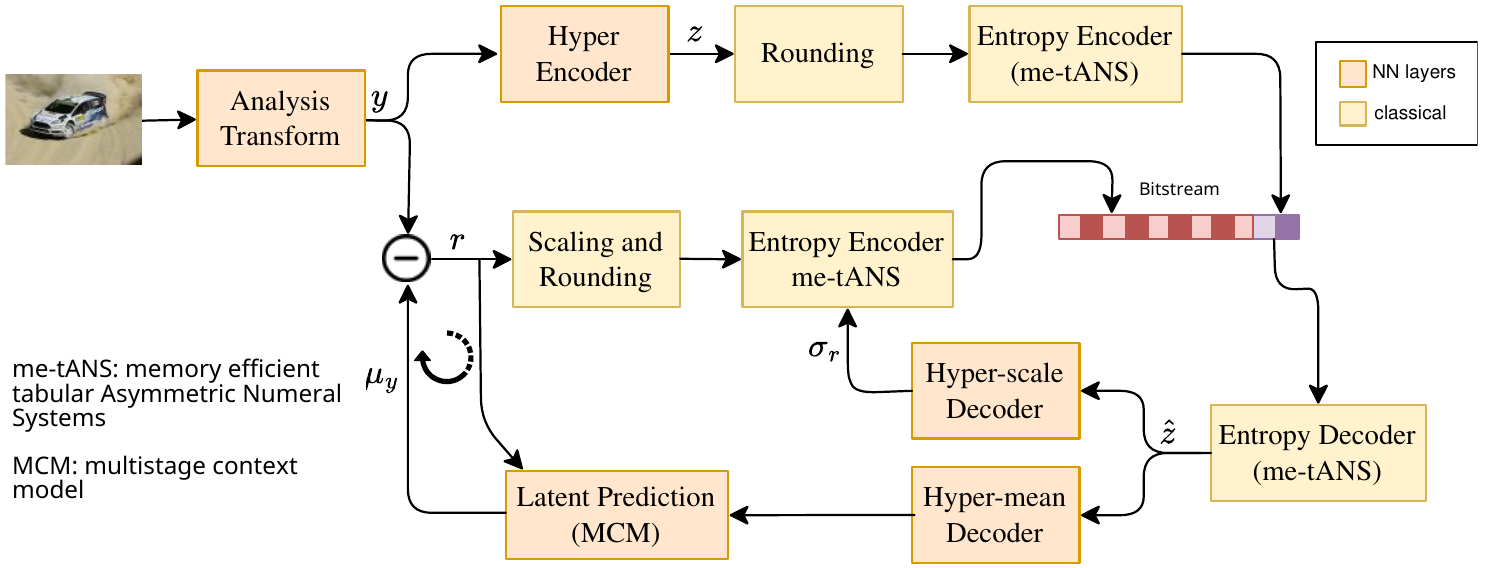
\includegraphics[width=1\linewidth]{img/encongdingJPEGAI.png}
    \caption{Schema della fase di encoding}
    \label{fig:encodingJPEGAI}
\end{figure}
\paragraph{Fase di Decoding}
Nella fase di decoding (vedi fig. \ref{fig:decodingJPEGAI}) avviene il processo inverso: inizialmente viene fatta la decodifica delle informazioni ausiliari $\hat{z}$, che vengono passate all'hyper-decoder (identico a quello della fase di encoding); i parametri calcolati da quest'ultimo vengono usati per decodificare in modo più efficiente i residui, ottenndo $\hat{r}$. Attraverso un modulo di latent prediction vengono nuovamente stimati $\hat{y}$, che è ricevuta dalla synthesis transform che produce un'immagine partendo dalla rappresentazione latente ricevuta.
\begin{figure}
    \centering
    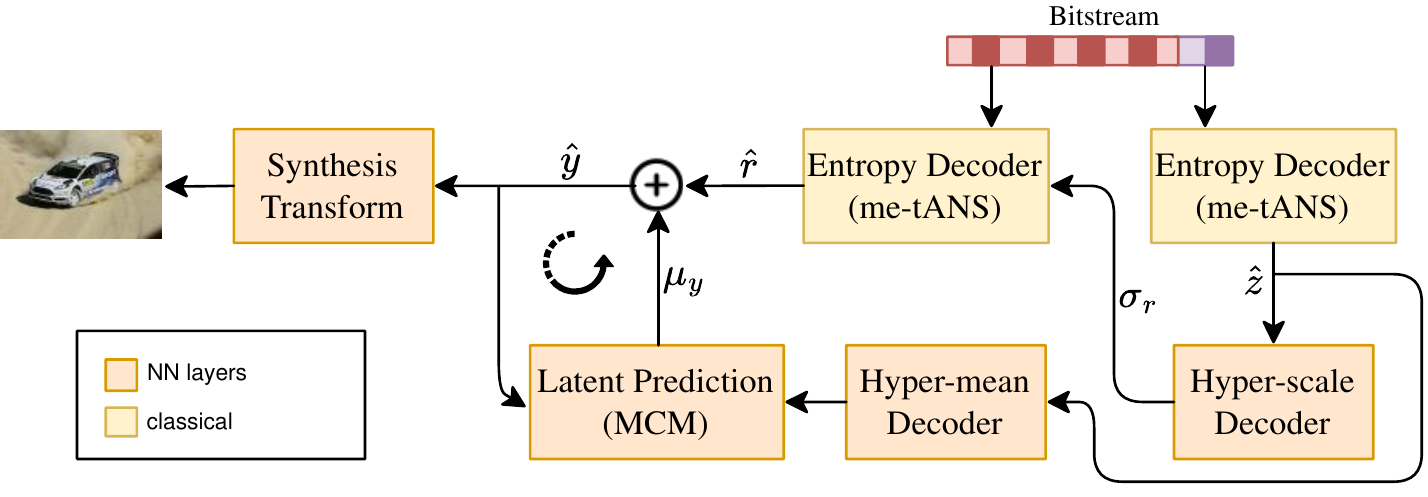
\includegraphics[width=1\linewidth]{img/decodingJPEGAI.png}
    \caption{Fase di Decoding di JPEG AI}
    \label{fig:decodingJPEGAI}
\end{figure}
\paragraph{Risultati ottenuti da JPEG AI}\label{par:riep}
I primi esperimenti hanno riscontrato risultati promettenti: con le prime versioni delle implementazioni JPEG AI è riuscito a raggiungere un BD-rate gain (\textit{Bjøntegaard-Delta Rate}, una metrica per la valutazione dell'efficienza di compressione) del 28\% \cite{ascenso2023jpegAI}  rispetto a VVC Intra (lo standard attdi compressione più effciente attualmente disponibile) usando la configurazione più semplice "\textit{tools-off}" senza ottimizzazioni avanzate. Inoltre è stato notato anche un miglioramento nella qualità soggettiva a parità di bitrate \cite{ascenso2023jpegAI}, confermando il potenziale di questo strumento.
\subsection{Conseguenze sulla multimedia forensics}
La creazione di JPEG AI introduce nuove sfide nel campo della multimedia forensics. In \cite{hofer2024taxonomy} viene definito il termine \textit{miscompression} per indicare gli errori creati nella ricostruzione delle immagini che portano ad avere dettagli semantici diversi tra l'immagine reale e quella ricostruita.
Poichè l'architettura è simile a quella dei generatori di immagini sintetici, in \cite{cannas2024jpeg} viene spiegato come le immagini compresse con JPEG AI presentano artefatti simili a quelle false, che porta i detetctor esistenti a classificarli in modo errato rilevandole come immagini sintetiche.
In \cite{bergmann2025three} vengono proposti tre indizi forensi per il rilevamento e l'analisi di immagini compresse con JPEG AI: correlazioni di colore, quantizzazione nello spazio latente e analisi della rate-distortion.

